\documentclass[12pt,addpoints]{exam}
%\usepackage{enumitem}
\usepackage{amsfonts,amssymb,amsmath, amsthm}
\usepackage{graphicx}
\usepackage{systeme}
\usepackage{pgf,tikz,pgfplots}
\pgfplotsset{compat=1.15}
\usepgfplotslibrary{fillbetween}
\usepackage{mathrsfs}
\usetikzlibrary{arrows}
\usetikzlibrary{calc}
\usepackage{geometry}
\geometry{
	a4paper,
	total={170mm,257mm},
	left=20mm,
	top=20mm,
}
\date{May, 2023}
\pagestyle{headandfoot}
%\firstpageheadrule
\runningheader{4th Quarter Midterm Examination}{}{Page \thepage\ of \numpages}
\runningheadrule
\firstpagefooter{}{}{}
\runningfooter{By Aaron G.K.}{}{Page \thepage\ of \numpages}
\begin{document}
	\title{St John Baptist De La Salle Catholic School, Addis Ababa\\
		\large Grade 10 Physics Midterm Examination \\
		$4^\text{th}$ Quarter}
	\maketitle
	\begin{center}
		\fbox{\fbox{\parbox{6in}{\centering
					Notes, and use of other aids is \textbf{NOT} allowed.  Read all directions carefully and \textbf{write your answers in the answer sheet}.  To receive full credit, you must show all of your work.
	}}}	\end{center}
	{Name:\underline{\hspace{2in}}\text{     }{Roll Number:\underline{\hspace{0.5in}}\text{     }{Section:\underline{\hspace{0.3in}}{Time Allowed: \bf{60  minutes}}
				\subsubsection*{Multiple Choice Questions}
				\begin{questions}
					\question When light travels from medium A to medium B, it refracts towards the normal. Which of the following is true?
					\begin{choices}
						\choice Light travels faster in medium B than medium A.
						\choice The wavelength of light in medium B is larger than its wavelength in medium A.
						\choice The frequency of light in medium B is larger than its frequency in medium A.
						\choice The refractive index of medium B is greater than that of medium A's.
					\end{choices}
					\textbf{Answer: D}
					\question If the amplitude of the electric field on an electromagnetic wave is $3\times10^{6}V/m$, what is the amplitude of the magnetic field?($c=3\times10^{8}m/s$) \\
					\begin{oneparchoices}
						\choice $3\times10^2T$
						\choice $1\times10^6G$
						\choice $3\times10^{2}G$
						\choice $1\times10^{-2}T$	
					\end{oneparchoices}
					\\ \textbf{Answer: D}	
					\question Why are ELF radio waves used for communication instead of say, UHF or VHF, radio signals?
					\begin{choices}
						\choice ELF radio waves have larger wavelengths which implies that they are able to carry more information per pulse to transfer into submarines.
						\choice ELF radio waves have larger frequencies which implies that they are able to carry more information per pulse to transfer into submarines.
						\choice ELF radio waves have larger wavelengths which implies that they are able to travel deeper which makes them ideal communicators.
						\choice ELF radio waves have larger speeds compared to UHF \& VHF signals which make the communication smoother.
					\end{choices}
					\textbf{Answer: C}
					\question When light is used in microscopy, the detail it can show is limited by its wavelength. What is the smallest detail visible by a light whose frequency is $1.5\times10^{15}Hz$? \\
					\begin{oneparchoices}
						\choice $2.0\times10^{-7}nm$
						\choice $200nm$
						\choice $250nm$
						\choice We can't say for sure.
					\end{oneparchoices}
					\\ \textbf{Answer: B}
					\question A radar is used to monitor the impacts on the surface of an asteroid nearby Earth. The asteroid is about $1.08\times10^{11}km$ away from Earth. How long does it take for a pulse emitted from the radar to reflect back to it?\\
					\begin{oneparchoices}
						\choice 1 hour
						\choice 100 hours
						\choice 200 hours
						\choice 3600 hours
					\end{oneparchoices}
					\\ \textbf{Answer: C}
					\question A light ray is traveling through the interface between a glass and water emerging from the glass($n=\dfrac{8}{3}$) to water($n=1.33$). Which of the following is true if the light was incident at an angle of $30^0$, which of the following is true?
					\begin{choices}
						\choice The light ray bends towards the perpendicular to the interface.
						\choice $30^0$ is the critical angle for the light.
						\choice If the angle of incidence was smaller than $30^0$, the light ray would reflect back instead of refracting.
						\choice The wavelength and the speed of the ray will decrease when entering water.
					\end{choices}
					\textbf{Answer: B}
					\question Unlike other types of mirrors, the images formed by plane mirrors are \\
					\begin{oneparchoices}
						\choice Virtual
						\choice Right to left inverted
						\choice Upright
						\choice All
					\end{oneparchoices}
					\\ \textbf{Answer: D}
					\question We have been describing electromagnetic waves as being self-propagating unlike other waves such sound. What do we mean by that?
					\begin{choices}
						\choice We mean that electromagnetic waves do not need medium to travel through because they have a special medium called the luminiferous ether to help them travel.
						\choice We mean that electromagnetic waves are transverse disturbances while waves like sound are longitudinal.
						\choice We mean that electromagnetic waves need media to travel through while other waves don't.
						\choice We mean that electromagnetic waves don't need media to travel through because they are disturbances of electromagnetic fields themselves that travel away from source.
					\end{choices} 
					\textbf{Answer: D}
					\question $\gamma$ rays and X rays are similar in the sense that both are very energetic, high frequency waves that usually offer similar applications. How are they different?
					\begin{choices}
						\choice X rays are formed only by the process of the bremsstrahlung while $\gamma$ rays are only produced by thermal agitation.
						\choice Although they have some overlapping frequency ranges, X rays generally have larger frequencies $\gamma$ rays.
						\choice X rays can be produced by electronic transition while $\gamma$ rays usually require a nuclear process.
						\choice X rays and $\gamma$ rays are identical except for their difference in frequency.
					\end{choices}
					\textbf{Answer: C}
					\question If you wish to detect details of the size of atoms (about 1A$^0$) with electromagnetic radiation, which of the following electromagnetic waves would you use? \\
					\begin{oneparchoices}
						\choice Visible light
						\choice X rays
						\choice Radio waves
						\choice Infrared waves
					\end{oneparchoices}
					\\ \textbf{Answer: B}
					\question Which of the following electromagnetic waves is usually radiated during the thermal agitation of matter?\\
					\begin{oneparchoices}
						\choice Microwaves
						\choice Visible light
						\choice Infrared radiation
						\choice $\gamma$ rays
					\end{oneparchoices}
					\\ \textbf{Answer: A/C}
					\question Which of the following is \textbf{most} refracted when light from the sun is passing through the atmosphere? \\
					\begin{oneparchoices}
						\choice Violet visible light
						\choice Blue visible light
						\choice Infrared radiation
						\choice Ultraviolet radiation
					\end{oneparchoices}
					\\ \textbf{Answer: D}
					\question If there are two mirrors that are perpendicular to each other, what is the relationship between the incoming light ray and the outgoing reflected ray? They \\
					\begin{oneparchoices}
						\choice are parallel
						\choice are perpendicular
						\choice cross each other at $45^0$
						\choice diverge
					\end{oneparchoices}.
					\\ \textbf{Answer: A}
					\question What is the speed of light in water($n=1.33$)?\\
					\begin{oneparchoices}
						\choice $4.0\times10^{8}m/s$
						\choice $2.0\times10^{8}m/s$
						\choice $2.25\times10^{8}m/s$
						\choice $3.0\times10^{8}m/s$
					\end{oneparchoices}
					\\ \textbf{Answer: C}
					\question If a person is standing still in a swimming pool, their legs appear \noindent\rule{1.5cm}{0.4pt} when viewed from outside the pool.\\
					\begin{oneparchoices}
						\choice longer
						\choice shorter
						\choice the same size
						\choice invisible
					\end{oneparchoices}
					\\ \textbf{Answer: B}
					\subsubsection*{Workout Problems}
					\question Calculate the ratio of the highest to lowest frequencies of electromagnetic waves the eye can see, given the wavelength range of visible light is from 450 nm to 760 nm. Would we be able to observe and study human cells  which have an average diameter of about $100\mu m$? Why? \\ \\
					One of the frequencies is:
					$$f=\dfrac{c}{\lambda}$$
					$$f=\dfrac{3\times10^8m/s}{450\times10^{-9}m}=6.67\times10^{14}Hz$$
					The other is:
					$$f=\dfrac{c}{\lambda}$$
					$$f=\dfrac{3\times10^8m/s}{750\times10^{-9}m}=4\times10^{14}Hz$$
					The ratio can be calculated as follows;
					$$\dfrac{6.67\times10^{14}Hz}{4\times10^{14}Hz}=\dfrac{6.67}{4}$$
					Another - a much simpler way - to calculate the ratio is relating the two frequencies as a function of their wavelengths:
					$$\dfrac{f_1}{f_2}=\dfrac{\dfrac{c}{\lambda_1}}{\dfrac{c}{\lambda_2}}$$
					$$\dfrac{f_1}{f_2}=\dfrac{\lambda_2}{\lambda_1}$$
					$$\dfrac{f_1}{f_2}=\dfrac{750nm}{450nm}=\dfrac{750}{450}=\dfrac{15}{9}\approxeq\dfrac{6.67}{4}$$
					\question A scuba diver training in a pool looks at his instructor. What angle does the ray from the instructor’s face make with the perpendicular to the water at the point where the ray enters? The angle between the ray in the water and the perpendicular to the water is $30^0$(The diver is at a depth of 2m below the surface of the water and the instructor is 2m away from the normal).
					\begin{center}
						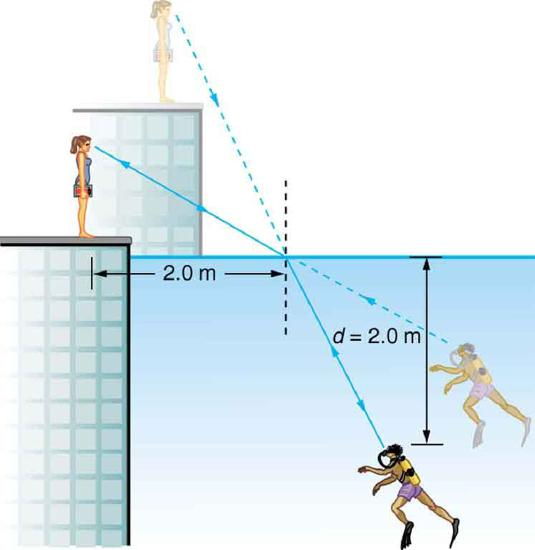
\includegraphics[scale=0.3]{1}
					\end{center}
					The angle given in the question is the angle of incidence. We are asked the angle of refraction. Despite the seemingly-intimidating nature of this question, it is quiet easy. We just have to use Snell's law.
					$$n_1\sin\theta_i=n_2\sin\theta_r$$
					Here, the first medium is water($n=\dfrac{4}{3}$) and the second medium is air($n=1$).
					$$\dfrac{4}{3}\sin30^0=(1)\sin\theta_r$$
					$$\sin\theta=\dfrac{2}{3}$$
					$$\theta=\arcsin\dfrac{2}{3}$$
					\question Light traveling from water($n=1.33$) to a some transparent stone strikes the surface at an incident angle of $60.0^0$ and has an angle of refraction of $37.0^0$.
					\begin{itemize}
						\item What is the speed of light in the stone? \\ \\
						To answer this, we first need to find the refractive index of the stone. To do that, we use Snell's law. The first medium is water and the second medium is the stone and we have been given the angles of incidence and reflection.
						$$n_1\sin\theta_i=n_2\sin\theta_r$$	
						$$(\dfrac{4}{3})\sin60^0=n_2\sin37^0$$
						$$(\dfrac{4}{3})\dfrac{\sqrt{3}}{2}=n_2(\dfrac{3}{5})$$
						$$n_2=\dfrac{10\sqrt{3}}{9}$$
						Now that we have the refractive index, we can work out the speed of light in this medium.
						$$n=\dfrac{c}{v}\implies v=\dfrac{c}{n}$$
						$$v=\dfrac{3\times10^{8}m/s}{\dfrac{10\sqrt{3}}{9}}$$
						\item What is the critical angle if light was to travel from the stone to water? \\ \\
						$$\sin\theta_c=\dfrac{n_2}{n_1}$$
						$$\theta_c=\arcsin\dfrac{n_2}{n_1}$$
						$$\theta_c=\arcsin\dfrac{\dfrac{4}{3}}{\dfrac{10\sqrt{3}}{9}}=\arcsin\dfrac{6}{5\sqrt{3}}$$
					\end{itemize}
					\question During normal beating, the heart creates a maximum 4.00-mV potential across 0.350 m of a person’s chest. If the EM wave created has a frequency of 7.00Hz,
					\begin{itemize}
						\item What is the maximum electric field strength created?
						We can find the electric field by using the voltage provided.
						$$E=\dfrac{V}{d}=\dfrac{4\times10^{-3}V}{0.35m}=1.14\times10^{-2}V/m$$
						\item What is the corresponding maximum magnetic field strength in the electromagnetic wave?
						$$E=cB\implies B=\dfrac{E}{c}=\dfrac{1.14\times10^{-2}V/m}{3\times10^{8}m/s}$$
						$$B=3.81\times10^{-11}T$$
					\end{itemize}
					\subsubsection*{Extra credit problems}
					\question A light ray entering an optical fiber surrounded by air is first refracted and then reflected as shown in the figure below. Show that if the fiber is made from crown glass($n=1.52$), any incident ray will be totally internally reflected.
					\begin{center}
						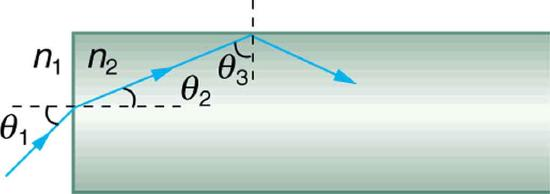
\includegraphics[scale=0.3]{2}
					\end{center}
					If the fiber is made of crown glass, the critical angle for the incident rays should be:
					$$\sin\theta_c=\dfrac{1.0}{1.52}$$
					$$\theta_c=\arcsin\dfrac{1.0}{1.52}=41.14^0$$
					For the incident ray to be totally internally reflected, $\theta_3>41.14^0$.  
					Since $$\theta_2+\theta_3=90^0\implies\theta_3=90^0-\theta_2$$. Thus, 
					$$90^0-\theta_2>41.14^0$$
					$$\theta_2<48.86^0$$
					However, we know that for any $\theta_1$ value, we can't have a $\theta_2$ value of $48.86^0$ because the highest value $\theta_2$ can have is less than $41.14^0$ and that is when $\theta_1\approxeq90^0$. Thus, any incident angle of $\theta_1$ will result in a total internal reflection.
				\end{questions}
			\end{document}